<<<<<<< HEAD
\section{Modeling}
\label{sec:compModel}

\section{Modeling}

Section outline:

\begin{enumerate}

\item Description of DCE and parameter estimation  
\item Description of auto ARIMA 
\subitem (this should be limited and explain it is meant to be out of the box) point at the paper for auto arima for more details.
\item Description of the two naive methods (random walk and mean), make sure to explain that these methods are naive and simple but not necessarily bad.
\item\cmark Add a section talking about evaluation methods i.e., MASE, this text is currently written and just sitting at the beginning of the results. 

\end{enumerate}

\subsection{Lorenz Method of Analogues (LMA)}
TODO:
\begin{enumerate}
\item update examples
\item remove section on RMSE
\item update figures
\end{enumerate}


 \subsubsection{Reconstructing hidden dynamics}



Delay-coordinate embedding allows one to reconstruct a system's full
state-space dynamics from a \emph{single} scalar time-series
measurement---provided that some conditions hold regarding that data.
Specifically, if the underlying dynamics and the measurement
function---the mapping from the unknown state vector $\vec{X}$ to the
scalar value $x$ that one is measuring---are both smooth and generic,
Takens~\cite{takens} formally proves that the delay-coordinate map
\[
F(\tau,m)(x) = ([x(t) ~ x(t+\tau) ~ \dots ~x(t+m\tau)])
\]
from a $d$-dimensional smooth compact manifold $M$ to ${Re}^{2d+1}$,
where $t$ is time, is a diffeomorphism on $M$---in other words, that
the reconstructed dynamics and the true (hidden) dynamics have the
same topology.

This is an extremely powerful result: among other things, it means
that one can build a formal model of the full system dynamics without
measuring (or even knowing) every one of its state variables.  This is
the foundation of the modeling approach that is used in this paper.
The first step in the process is to estimate values for the two free
parameters in the delay-coordinate map: the delay $\tau$ and the
dimension $m$.  We follow standard procedures for this, choosing the
first minimum in the average mutual information as an estimate of
$\tau$ \cite{fraser-swinney} and using the false-near(est) neighbor
method of \cite{KBA92}, with a threshold of 10\%, to estimate $m$.  A
plot of the data from Figure~\ref{fig:ipc}, embedded following this
procedure, is shown in Figure~\ref{fig:embedding}.


 \begin{figure}
   \centering
     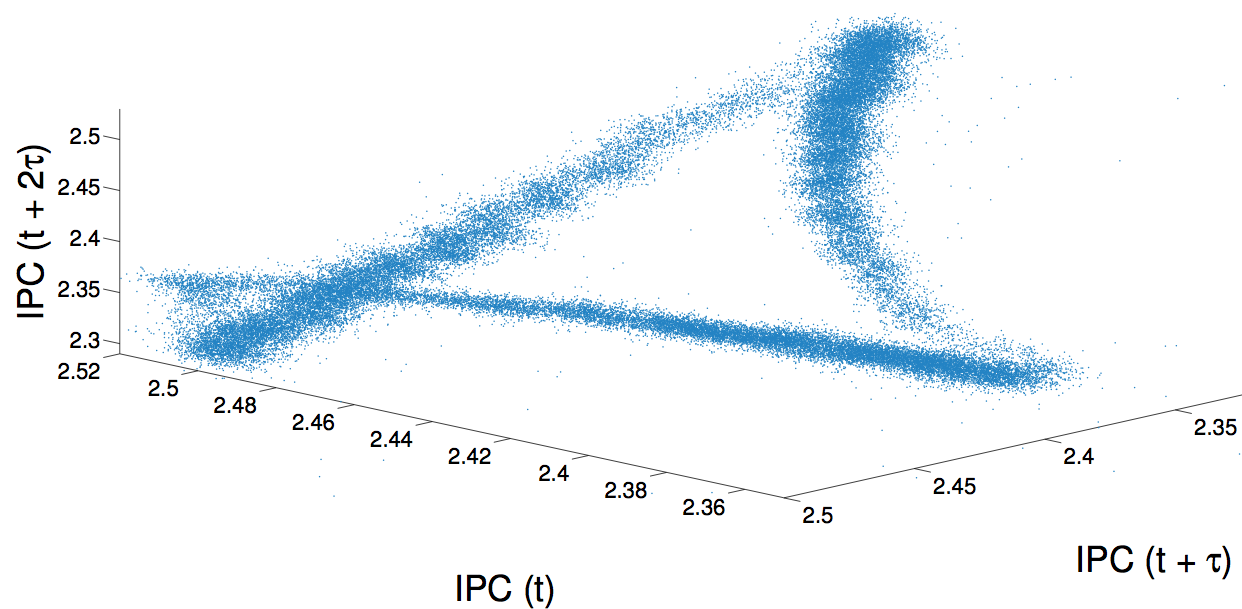
\includegraphics[width=\textwidth]{figs/colipc3d.png}
     \caption{[[Joshua:Perhaps add a similar graphic of \gcc to show contrast]]A 3D projection of a delay-coordinate embedding of the trace
 from Figure~\ref{fig:ipc} with a delay ($\tau$) of 100,000 instructions.
 }
 \label{fig:embedding}
 \end{figure}


%% can cut for space if need be:
The coordinates of each point on this plot are differently delayed
elements of the \col L2 cache miss rate time series
$y(t)$: that is, $y(t)$ on the first axis, $y(t+\tau)$ on the second,
$y(t+2\tau)$ on the third, and so on.
%% ...down to here.
Structure in these kinds of plots---clearly visible in
Figure~\ref{fig:embedding}---is an indication of
determinism\footnote{A deeper analysis of
  Figure~\ref{fig:embedding}---as alluded to on the previous
  page---supports that diagnosis, confirming the presence of a chaotic
  attractor in these cache-miss dynamics, with largest Lyapunov
  exponent $\lambda_1 = 8000 \pm 200$ instructions, embedded in a
  12-dimensional reconstruction space \cite{mytkowicz09}.}.  That
structure can also be used to build a forecast model.

% took out for space
 \subsubsection{LMA: Using dynamics in forecasting}

Given a nonlinear model of a deterministic dynamical system in the
form of a delay-coordinate embedding like Figure~\ref{fig:embedding},
one can build deterministic forecast algorithms by capturing and
exploiting the geometry of the embedding.  Many techniques have been
developed by the dynamical systems community for this purpose
(e.g.,~\cite{casdagli-eubank92,weigend-book}).  Perhaps the most straightforward
is the ``Lorenz method of analogues'' (LMA), which is essentially
nearest-neighbor prediction in the embedded state
space~\cite{lorenz-analogues}.  Even this simple algorithm---which
builds predictions by finding the nearest neighbor in the embedded
space of the given point, then taking that neighbor's path as the
forecast---works quite well on the trace in Figure~\ref{fig:ipc}, as
shown in Figure~\ref{fig:cachePredTS}.
%
%\begin{figure}[htbp]
%  \centering
%    \includegraphics[width=0.5\textwidth]{figs/%colCachePredTS}
%    \caption{A forecast of the last 4,000 points of the %signal in
%      Figure~\ref{fig:ipc} using an LMA-based strategy on the
%      embedding in Figure~\ref{fig:embedding}.  Red circles %and blue
%      $\times$s are the true and predicted values, %respectively;
%      vertical bars show where these values differ. }
%\label{fig:cachePredTS}
%\end{figure}
%
On the other hand, if we use the same approach to forecast the
processor load\footnote{Instructions per cycle, or IPC} of the {\tt
  482.sphinx3} program from the SPEC cpu2006 benchmark suite, running
on an Intel i7\textsuperscript{\textregistered}-based machine, the
prediction is far less accurate; see Figure~\ref{fig:predsphinx}.
%
%\begin{figure}[htbp]
%  \centering
%    \includegraphics[width=0.5\textwidth]{figs/%sphinxPredicTS}
%     \caption{An LMA-based forecast of the last 4,000 points %of a
%       processor-load performance trace from the {\tt %482.sphinx3}
%       benchmark.  Red circles and blue $\times$s are the %true and
%       predicted values, respectively; vertical bars show %where these
%       values differ.}
%\label{fig:predsphinx}
%\end{figure}

%Table~\ref{tab:PredError} presents detailed results about the prediction accuracy of this algorithm on four different examples: the {\tt col\_major} and {\tt 482.sphinx3} programs in Figures~\ref{fig:cachePredTS} and~\ref{fig:predsphinx}, as well as another simple microkernel that initializes the same matrix as {\tt col\_major}, but in row-major order, and another complex program ({\tt 403.gcc}) from the SPEC cpu2006 benchmark suite.  Both microkernels were run on the Intel Core Duo\textsuperscript{\textregistered} machine; both SPEC benchmarks were run on the Intel i7\textsuperscript{\textregistered} machine.  We calculated a figure of merit for each prediction as follows.  We held back the last $k$ elements\footnote{Several different prediction   horizons were analyzed in our experiment; the results reported in this paper are for $k$=4000} of the $N$ points in each measured time series, built the forecast model by embedding the first $N-k$ points, used that embedding and the LMA method to predict the next $k$ points, then computed the Root Mean Squared Error (RMSE) between the true and predicted signals: $$RMSE = \sqrt{\frac{\sum_{i=1}^k(c_i-\hat{p_i})^2}{k}}$$ To compare the success of predictions across signals with different units, we normalized RMSE as follows: $$nRMSE = \frac{RMSE}{X_{max,obs}-X_{min,obs}}$$
%
% The smaller the nRMSE, obviously, the more accurate the prediction.



%The results in Table~\ref{tab:PredError} show a clear distinction between the two microkernels, whose future behavior can be predicted effectively using this simple deterministic modeling strategy, and the more-complex SPEC benchmarks, for which this prediction strategy does not work nearly as well.
% Removed for space
% For both processor load (IPC) and memory usage (cache-miss rate),
% forecasts for {\tt 482.sphinx3} and {\tt 403.gcc} are much worse than
% for \verb|col_major| or \verb|row_major|.
%
This begs the question: If these traces all come from deterministic
systems---computers---then why are they not equally predictable?  Our
conjecture is that the sheer complexity of the dynamics of the SPEC
benchmarks running on the Intel i7\textsuperscript{\textregistered}
machine make them effectively impossible to predict.

%% [[If space: Add a segue sentence: next section uses permutation
%% entropy to explore that conjecture.]]

%\subsection{Comparing Prediction Accuracy}

\subsection{Autoregressive-integrated-moving average(ARIMA)}
\subsection{Naive: Random Walk and na\"ive}
\subsection{Prediction Accuracy: Mean Absolute Scaled Error (MASE)}

\begin{figure}[htbp]
  \centering
   \begin{subfigure}{0.49\textwidth}
    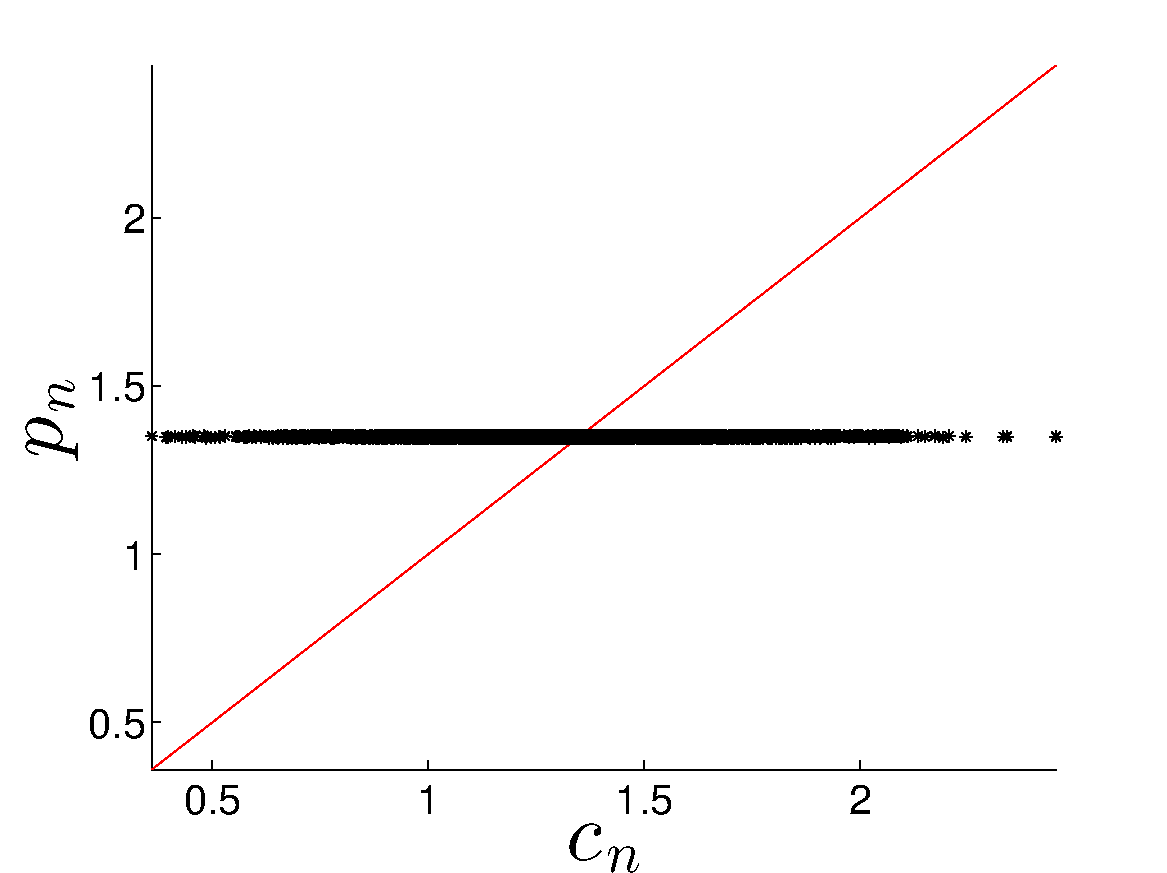
\includegraphics[width=\textwidth]{figs/gccMeanForecast}
    \caption{\gcc na\"ive }
    \label{fig:gccMEAN}
  \end{subfigure}%      
     \begin{subfigure}{0.49\textwidth}
    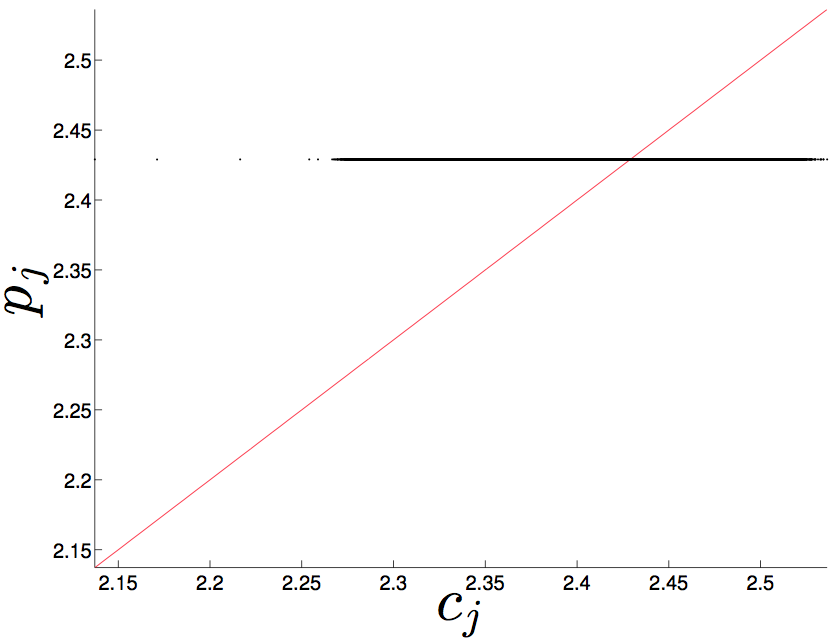
\includegraphics[width=\textwidth]{figs/colMeanForecast}
    \caption{\col na\"ive }
    \label{fig:gccMEAN}
  \end{subfigure}%    
  \\
  \begin{subfigure}{0.49\textwidth}
    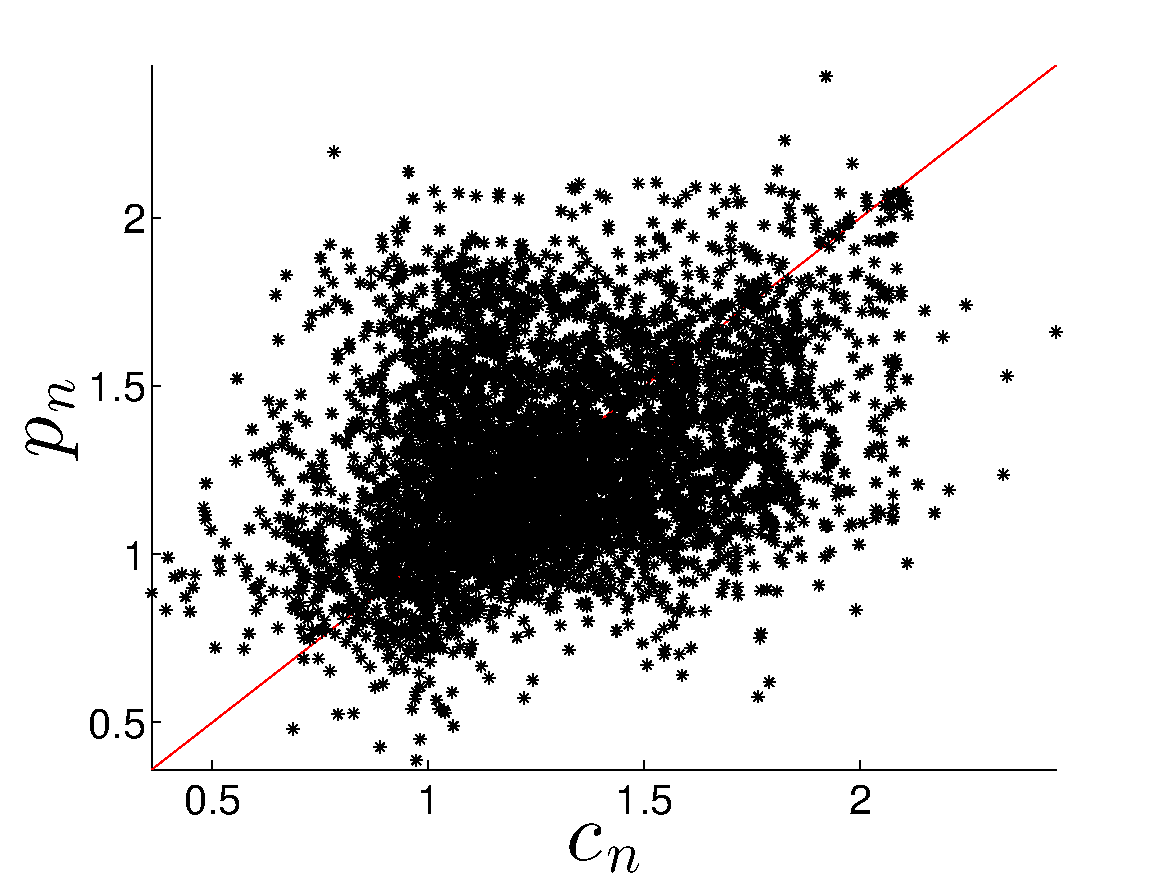
\includegraphics[width=\textwidth]{figs/gccARIMAForecast}
    \caption{\gcc ARIMA }
    \label{fig:gccARIMA}
  \end{subfigure}%
  \begin{subfigure}{0.49\textwidth}
    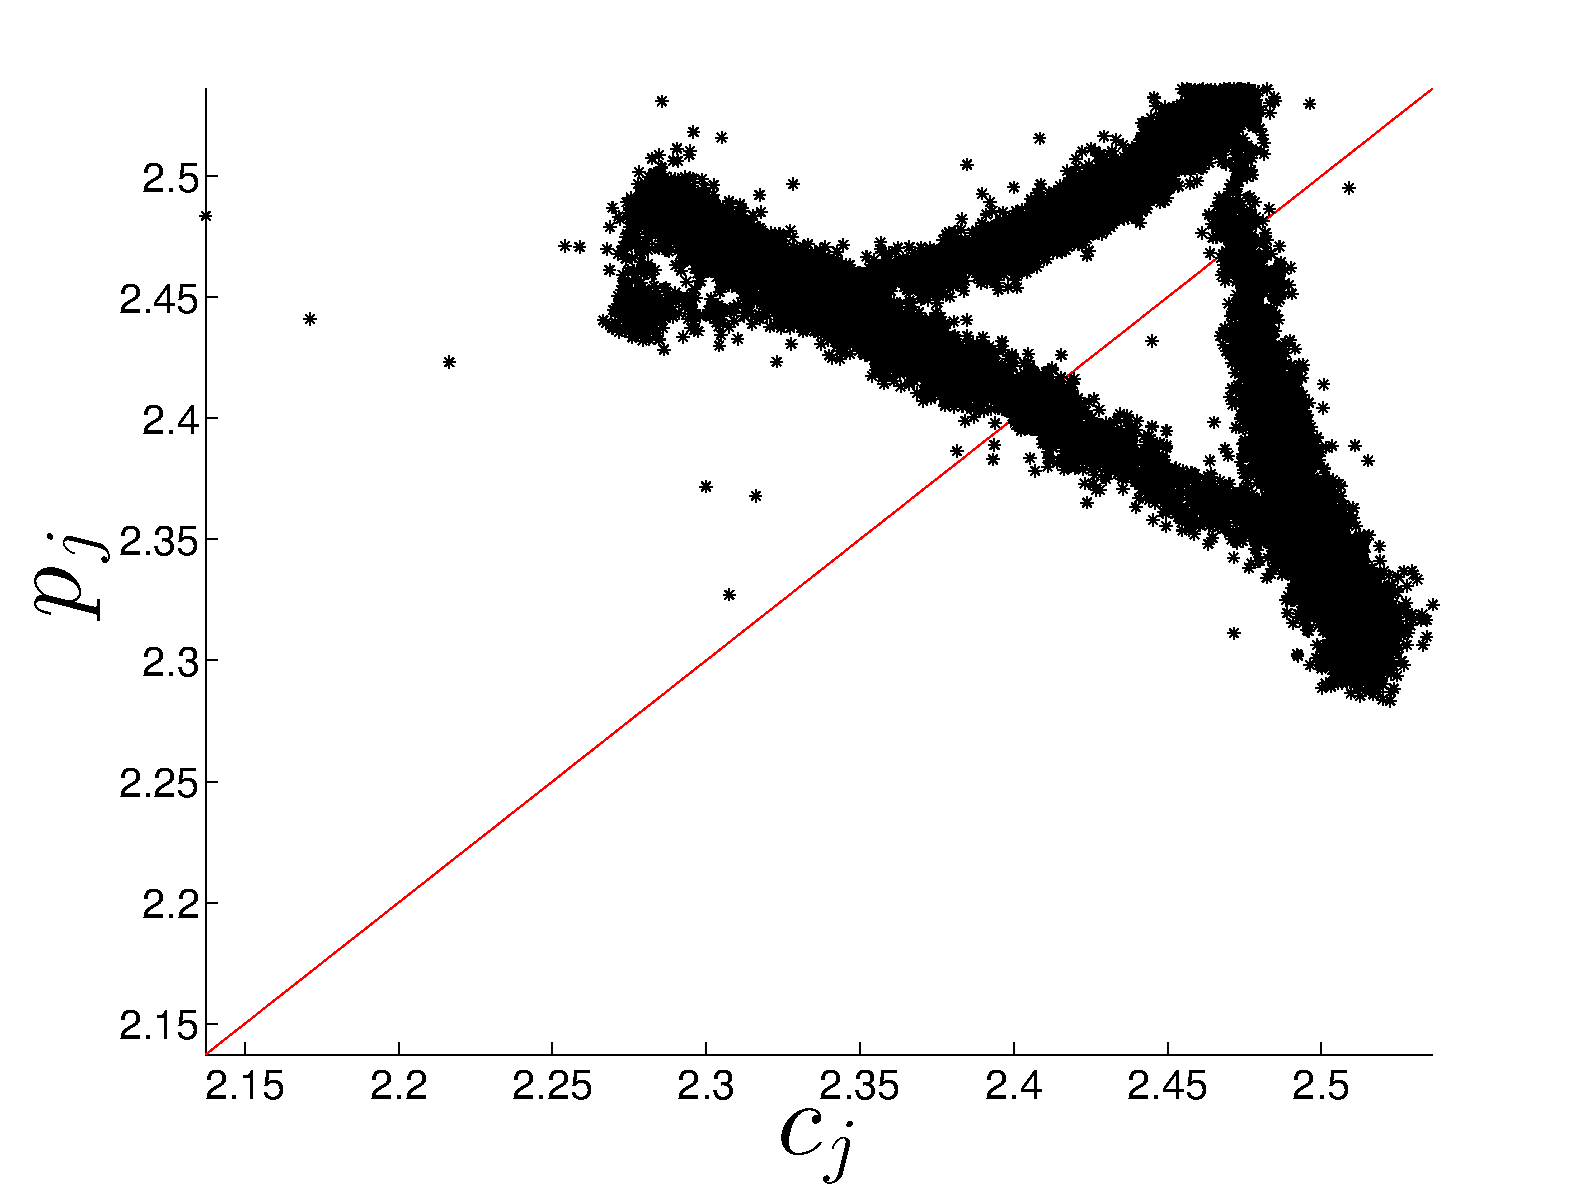
\includegraphics[width=\textwidth]{figs/colARIMAForecast}
    \caption{\col ARIMA}
    \label{fig:colARIMA}
  \end{subfigure}
  \\
      \begin{subfigure}{0.49\textwidth}
    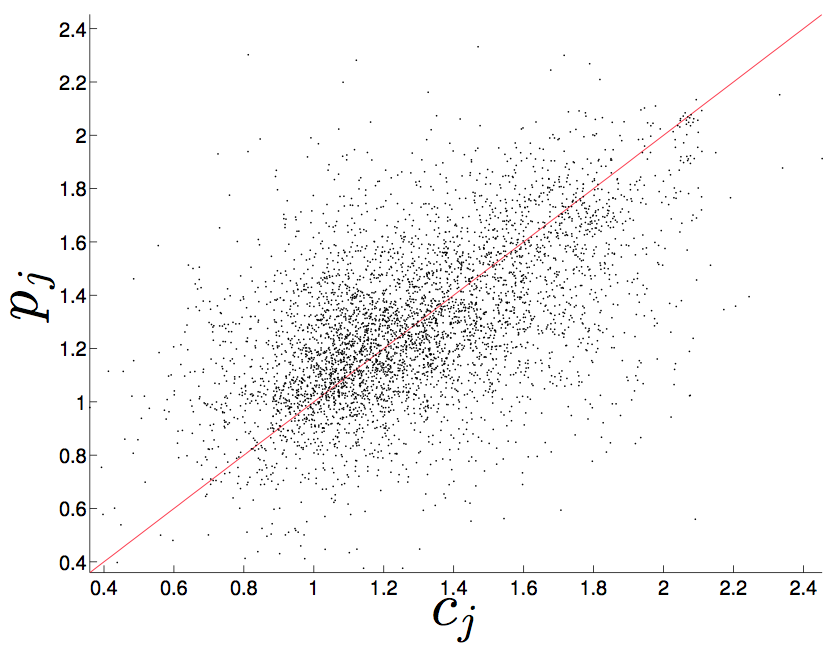
\includegraphics[width=\textwidth]{figs/gccLMAForecast}
    \caption{\gcc LMA}
    \label{fig:gccLMA}
  \end{subfigure}  
    \begin{subfigure}{0.49\textwidth}
    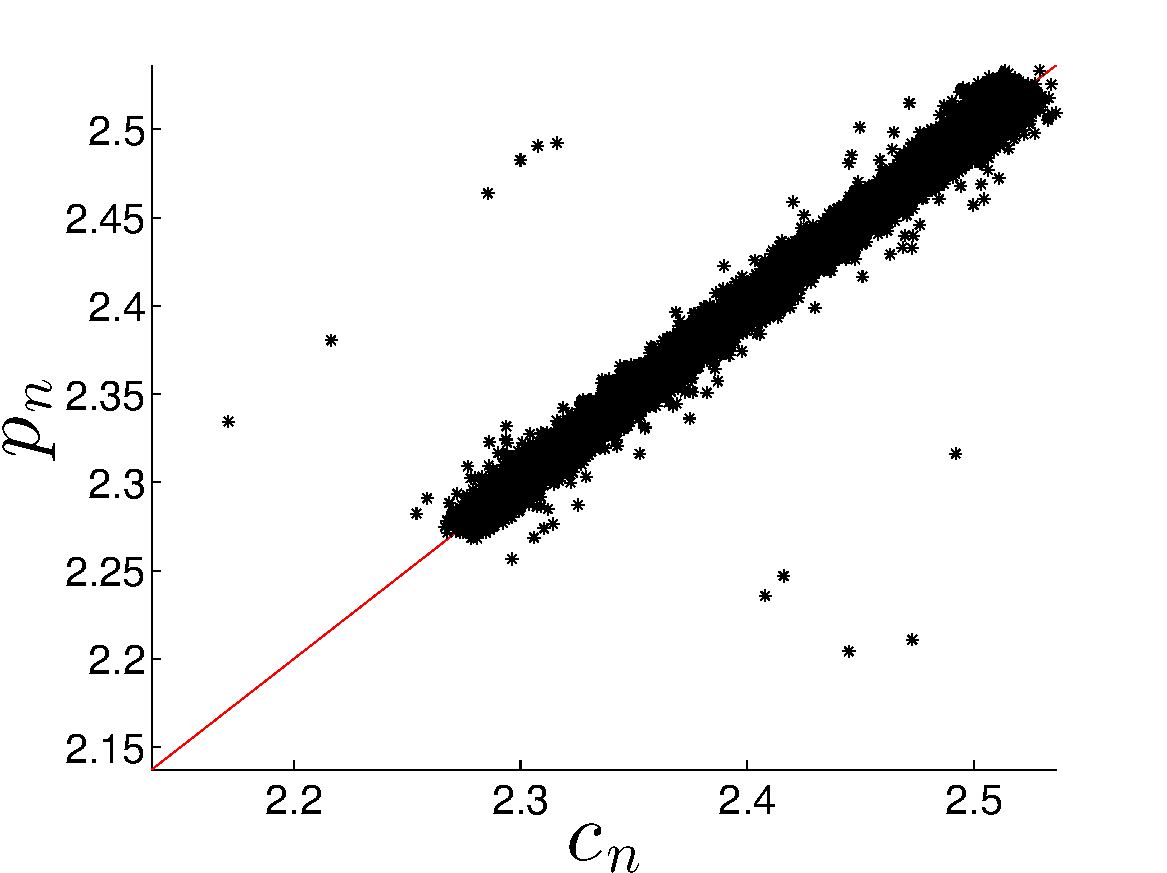
\includegraphics[width=\textwidth]{figs/colLMAForecast}
    \caption{\col LMA}
    \label{fig:colLMA}
  \end{subfigure}

  
  %\begin{subfigure}{0.5\textwidth}
  %  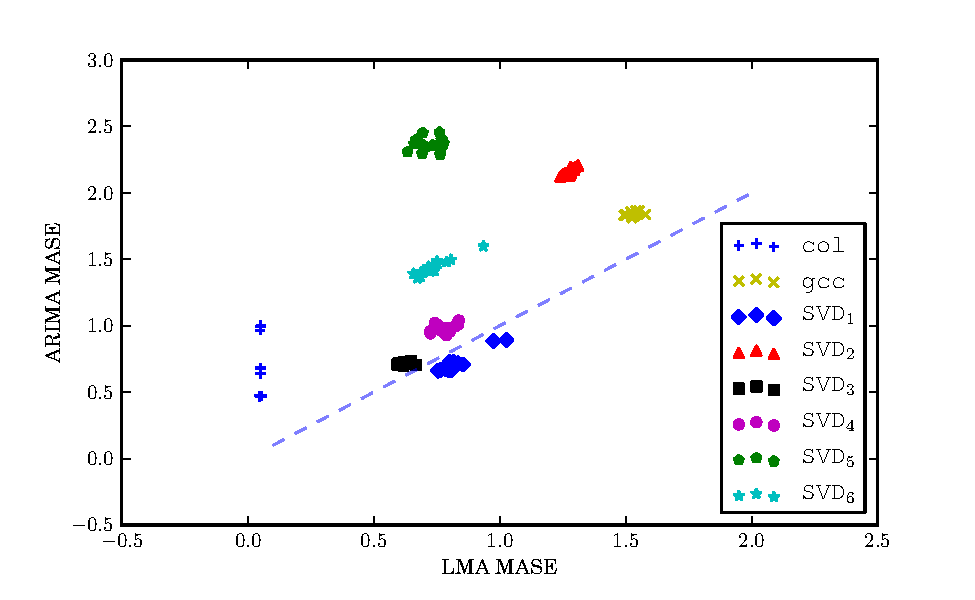
\includegraphics[width=1.0\textwidth]{figs/LMA_vs_ARIMA}
   \caption{
For each of these, we plot the predicted value $p_n$ against the correct value $c_n$. On this type of plot a perfect prediction lies exactly on the diagonal, that is the line $p_n = c_n$, e.g., \ref{fig:colLMA} is a near perfect prediction where-as \ref{fig:gccARIMA} is a very poor prediction. }\label{fig:gcc_vs_col}  
  %\end{subfigure}
\end{figure} 
In order to analyze correctness of each prediction we split each time series into two pieces: the first 90\% referred to as the ``learning" or ``training" signal, $\{X_{i,obs}\}_{i=1}^{n}$ and the last 10\% known as the ``test" or ``correct" signal $\{c_j\}_{j=n+1}^{k+n+1}$. The learning signal is used to train an initial model (e.g., LMA or ARIMA) as described in Section \ref{sec:compModel}. The test signal is used both to assess the models forecasting accuracy and for any refitting that may be necessary. In particular, we perform $k$ 1-step predictions, after each 1-step prediction\footnote{We would like to note that this rebuilding occurs due to a problem with ARIMA models converging to a mean prediction if too long of a prediction horizon is used, this is not a handicap of either LMA or na\"ive.} we append the training signal with the next point in the correct signal $c_j$, refit the model taking into account the new system measurement and perform another prediction. This is repeated $k$ times to obtain $\{p_j\}_{j=n+1}^{k+n+1}$.

As a figure of merit we calculate the Mean Absolute Squared Error (MASE)\cite{MASE} between the true and predicted signals: 
%In order to compare the resulting forecasts we calculate the Mean Absolute Squared Error (MASE)\cite{MASE} between the true and predicted signals:
$$MASE = \sum_{j=n+1}^{k+n+1}\frac{|c_j-p_j| }{\frac{k}{n-1}\sum^n_{i=2}|X_{i,obs}-X_{i-1,obs}|}$$
The scaling term for MASE:
$$\frac{1}{n-1}\sum^n_{i=2}|X_{i,obs}-X_{i-1,obs}|$$ 
is the average in-sample forecast error for a random walk prediction $(p_i=X_{i-1,obs})$. This error method was introduced in \cite{MASE} as a ``generally applicable measurement of forecast accuracy without the problems seen in the other measurements." The major advantage of MASE is that it allows fair comparison across methods, prediction horizons and varying signal scales. When a forecast results in a $MASE<1$ this means that the prediction method gave, on average, smaller errors than the 1-step errors from the in-sample random walk forecast strategy. Analogously, $MASE>1$ means that the prediction method did worse, on average than the 1-step errors for the in-sample random walk forecast strategy. In Table \ref{tab:error} we provide the distribution [[Joshua: Ryan, Is this the right word? we give mean $\pm$ std. dev but some have very skewed right tails]]  of MASEs for each of the 8 signals and 3 prediction strategies, these are averaged over 15 runs of each type (signal + method). [[and cherry pick a few examples of \gcc and \col to put in the text For comparison Table \ref{tab:error} also has the distribution of weighted permutation entropies for word lengths of $l=6$.]]







% took out for space

